Анализ данных будет проведен при помощи языка программирования Python3. Данный язык был выбран по нескольким причинам:
\begin{description}[font=$\bullet$]
\item большое количество модулей для анализа данных;
\item подробная документация как языка, так и его модулей;
\item удобство и простота работы с данными в форматах csv, xlsx;
\item множество встроенных функций и выразительность языка.
\end{description}



\section{Обзор признаков}
В данном наборе данных представлена информация о случаях схода составов с рельс по причине излома боковой рамы вагона.\\
Набор данных содержит следующие признаки:
\begin{description}[font=$\bullet$]
\item дата --  дата происшествия;
\item кол-во вагонов -- кол-во вагонов в составе (без локомотивов);
\item максимальное число вагонов в сходе -- кол-во вагонов с конца до сшедшего поезда;
\item общее кол-во вагонов -- кол-во вагонов в составе (с локомотивами);
\item кол-во сошедших вагонов -- целевая переменная; кол-во вагонов, сшедших с рельс;
\item скорость -- средняя скорость состава;
\item вес -- масса состава, включая груз, выраженная в тоннах;
\item загрузка -- отношение текущего веса к максимальному весу;
\item стрелочный перевод -- наличие стрелочного перевода в месте схода;
\item кривизна -- обратная величина к радиусу кривизны;
\item профиль пути -- знак величины определяет направление (положительный, если подъем и отрицательный, если спуск);
\item Режим движения -- дискретная величина, обозначающая тягу, выбег, торможение;\\
\end{description}
Вывод первых пяти записей из набора, таблица разделена на две части:
\begin{table}[H]
    \resizebox{\textwidth}{!}{%
        \begin{tabular}{c}
            \begin{tabular}{|c|c|c|c|c|c|}
                \hline
                № & Дата & Кол-во вагонов & Макс. число вагонов в сходе & Общее кол-во вагонов & Кол-во сшедших вагонов \\ \hline
                1 & 2013-01-08 & 56.0 & 19.0 & 58.0 & 1 \\ \hline
                2 & 2013-01-09 & 60.0 & 25.0 & 62.0 & 1 \\ \hline
                3 & 2013-01-10 & 60.0 & 4.0 & 64.0 & 1 \\ \hline
                4 & 2013-01-12 & 66.0 & 63.0 & 68.0 & 21 \\ \hline
                5 & 2013-01-19 & 67.0 & 34.0 & 69.0 & 1 \\ \hline
            \end{tabular}\\\\
            \begin{tabular}{|c|c|c|c|c|c|c|c|}
                \hline
                № & Скорость & Вес & Загрузка & Стрелочный перевод & Кривизна & Профиль пути & Режим движения \\ \hline
                1 & 57.0 & 3402.0 & 0.547101 & 0 & 0.000000 & 0.0007 & NaN \\ \hline
                2 & 72.0 & 4082.0 & 0.652657 & 0 & 0.000000 & 0.0009 & NaN \\ \hline
                3 & 15.0 & 4420.0 & 0.734300 & 0 & 0.001639 & NaN & 3.0 \\ \hline
                4 & 67.0 & 5699.0 & 0.918094 & 0 & 0.002326 & 0.0060 & NaN \\ \hline
                5 & 69.0 & 5854.0 & 0.932944 & 0 & 0.000000 & 0.0006 & 2.0 \\ \hline
            \end{tabular}
        \end{tabular}
    }
    \captionof{table}{первые 5 записей в наборе данных}
    \label{tab:first_5_records}
\end{table}


\section{Описательные статистики}

Мощность выборки равна 56, при этом в записях содержится существенное количество пропусков.
%Определим размеры выборки:
%\mint{python}|print("shape of data frame:", df.shape)|
%\mint{text}|> shape of data frame: (56, 12)|

%Выведем названия факторов:
%\mint{python}|print(df.columns)|
%\begin{minted}[fontsize=\footnotesize]{text}
%> Index(['Дата', 'Количество вагонов', 'Макс. число вагонов в сходе',
%'Общее количество вагонов', 'Количество сшедших вагонов', 'Скорость',
%'Вес', 'Загрузка', 'Стрелочный перевод', 'Кривизна', 'Профиль пути',
%'Режим движения'],
%dtype='object')
%\end{minted}

Вывод описательных статистик для набора данных (примечание: признак 'Дата' исключен):\\
\begin{table}[H]
    \resizebox{\textwidth}{!}{%
    \begin{tabular}{c}
        \begin{tabular}{|c|c|c|c|c|c|}
            \hline
            & Кол-во вагонов & Макс. число вагонов в сходе & Общее кол-во вагонов & Кол-во сшедших вагонов & Скорость \\ \hline
            count & 54.000000 & 51.000000 & 54.000000 & 56.000000 & 53.000000 \\ \hline
            mean & 63.870370 & 37.137255 & 66.407407 & 3.875000 & 49.150943 \\ \hline
            std & 9.790342 & 21.543463 & 10.053665 & 6.081455 & 18.450971 \\ \hline
            min & 24.000000 & 2.000000 & 26.000000 & 1.000000 & 9.000000 \\ \hline
            25\% & 60.000000 & 17.500000 & 62.500000 & 1.000000 & 35.000000 \\ \hline
            50\% & 66.000000 & 43.000000 & 68.000000 & 1.000000 & 51.000000 \\ \hline
            75\% & 68.000000 & 56.500000 & 71.750000 & 2.250000 & 64.000000 \\ \hline
            max & 96.000000 & 72.000000 & 100.000000 & 26.000000 & 78.000000 \\ \hline
        \end{tabular}\\\\
        \begin{tabular}{|c|c|c|c|c|c|c|}
            \hline
            & Вес & Загрузка & Стрелочный перевод & Кривизна & Профиль пути & Режим движения \\ \hline
            count & 54.000000 & 54.000000 & 56.000000 & 46.000000 & 44.000000 & 33.000000 \\ \hline
            mean & 5126.629630 & 0.817678 & 0.107143 & 0.000806 & -0.000384 & 1.666667 \\ \hline
            std & 1438.743887 & 0.243936 & 0.312094 & 0.001171 & 0.005689 & 0.777282 \\ \hline
            min & 998.000000 & 0.179710 & 0.000000 & 0.000000 & -0.011500 & 1.000000 \\ \hline
            25\% & 4155.500000 & 0.690451 & 0.000000 & 0.000000 & -0.004750 & 1.000000 \\ \hline
            50\% & 5722.000000 & 0.925519 & 0.000000 & 0.000000 & 0.000000 & 1.000000 \\ \hline
            75\% & 6010.250000 & 0.995586 & 0.000000 & 0.001479 & 0.001875 & 2.000000 \\ \hline
            max & 8806.000000 & 1.076087 & 1.000000 & 0.005000 & 0.010900 & 3.000000 \\ \hline
        \end{tabular}
    \end{tabular}
}
\captionof{table}{описательные статистики}
\label{tab:basic_stats}
\end{table}

Следует отметить, что такие признаки как: 'Режим движения', 'Кривизна', 'Профиль пути' имеют наибольшее количество пропусков в данных: $41\%$, $17\%$, $21\%$ пропусков соответственно.



\section{Корреляция признаков}

Построим матрицу корреляции признаков:
%\begin{minted}{python}
%corrmat = df.corr()
%f, ax = plt.subplots(figsize=(12, 9))
%sns.heatmap(corrmat, vmax=.8, square=True)
%\end{minted}

\begin{figure}[H]
\begin{center}
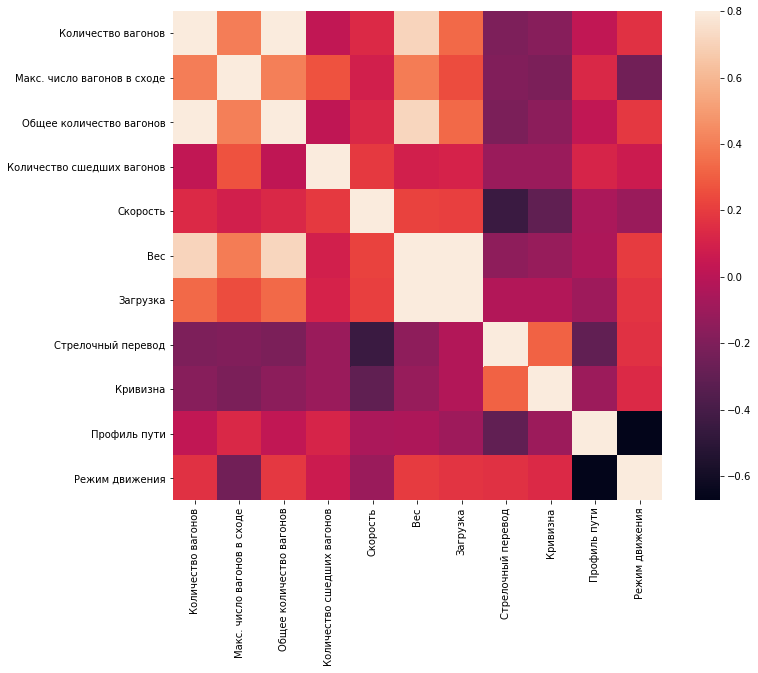
\includegraphics[width=0.85\linewidth]{src/img/df_corr}
\caption{Корреляция признаков}
\label{fig:df_corr}
\end{center}
\end{figure}

Из рисунка \ref{fig:df_corr} видно, что признаки 'Количество вогонов' и 'Общее число вагонов' имеют сильную корреляцию, что можно объяснить тем, что общее число вагонов равно количеству вагонов плюс количество локомотивов, при этом количество локомотивов в составах как правило равняется двум, следовательно получается функциональная зависимость. Также можно заметить, что признаки 'Вес' и 'Загрузка' сильно коррелируют. Менее сильная корреляция наблюдается у признаков 'Вес' и 'Общее число вагонов'. Заметим, что у 'Профиль пути' и 'Режим движения' наблюдается сильная обратная корреляция. Многие зависимости можно нетрудно объяснить: чем больше вагонов в составе, тем больше вес, чем больший вес, тем, как правило, большая загруженность. Таким образом, можно прийти к выводу, что в данные в наборе избыточны, поскольку несколько признаков несут одинаковое количество информации. Поэтому эти зависимости приводят к проблеме мультиколлинеарности, что приведет к эффекту переобучения в линейных моделях. Для решения данной проблемы нужно исключить избыточные признаки.



\section{Пропуски в данных}

Из таблицы \ref{tab:basic_stats} по строке 'count' видно, что в последних трёх признаках присутствуют пропуски в данных. Для решения проблемы пропусков в данных существует ряд методов:

\begin{description}[font=$\bullet$]
    \item удалить все записи из используемого в модели подмножества признаков, в которых есть хотя бы одно пустое поле. При использовании этого метода для данного набора данных существует риск того, что оставшегося множества записей не хватит для получения приемлемого качества построенной модели;
    \item заменить пропуски на средние значение по признаку;
    \item заменить пропуски на медианные значение по признаку. В отличие от среднего значения замена на медианное позволяет избежать сильного влияния выбросов на итоговое значение;
    \item заменить пропуски на крайне большие значения, если в качестве модели так или иначе используется структура данных дерево. Таким образом, все записи, имеющие пропуски будут выделены в отдельную ветку дерева;
    \item заменить пропуски нулевыми значениями, таким образом для логистической регрессии пропуски в данных не будут влиять на предсказанные значения.
\end{description}
При решении данной задачи будет использован метод удаления записей с пропусками. Замена значений на медианное, среднее для данного набора данных может оказаться не оптимальным выбором, поскольку мощность выборки не велика.



\section{Экстремальные значения}

Для поиска выбросов построим графики, изображающие отношения между парами признаков, и гистограммы распределений.\\

\begin{figure}[H]
\begin{center}
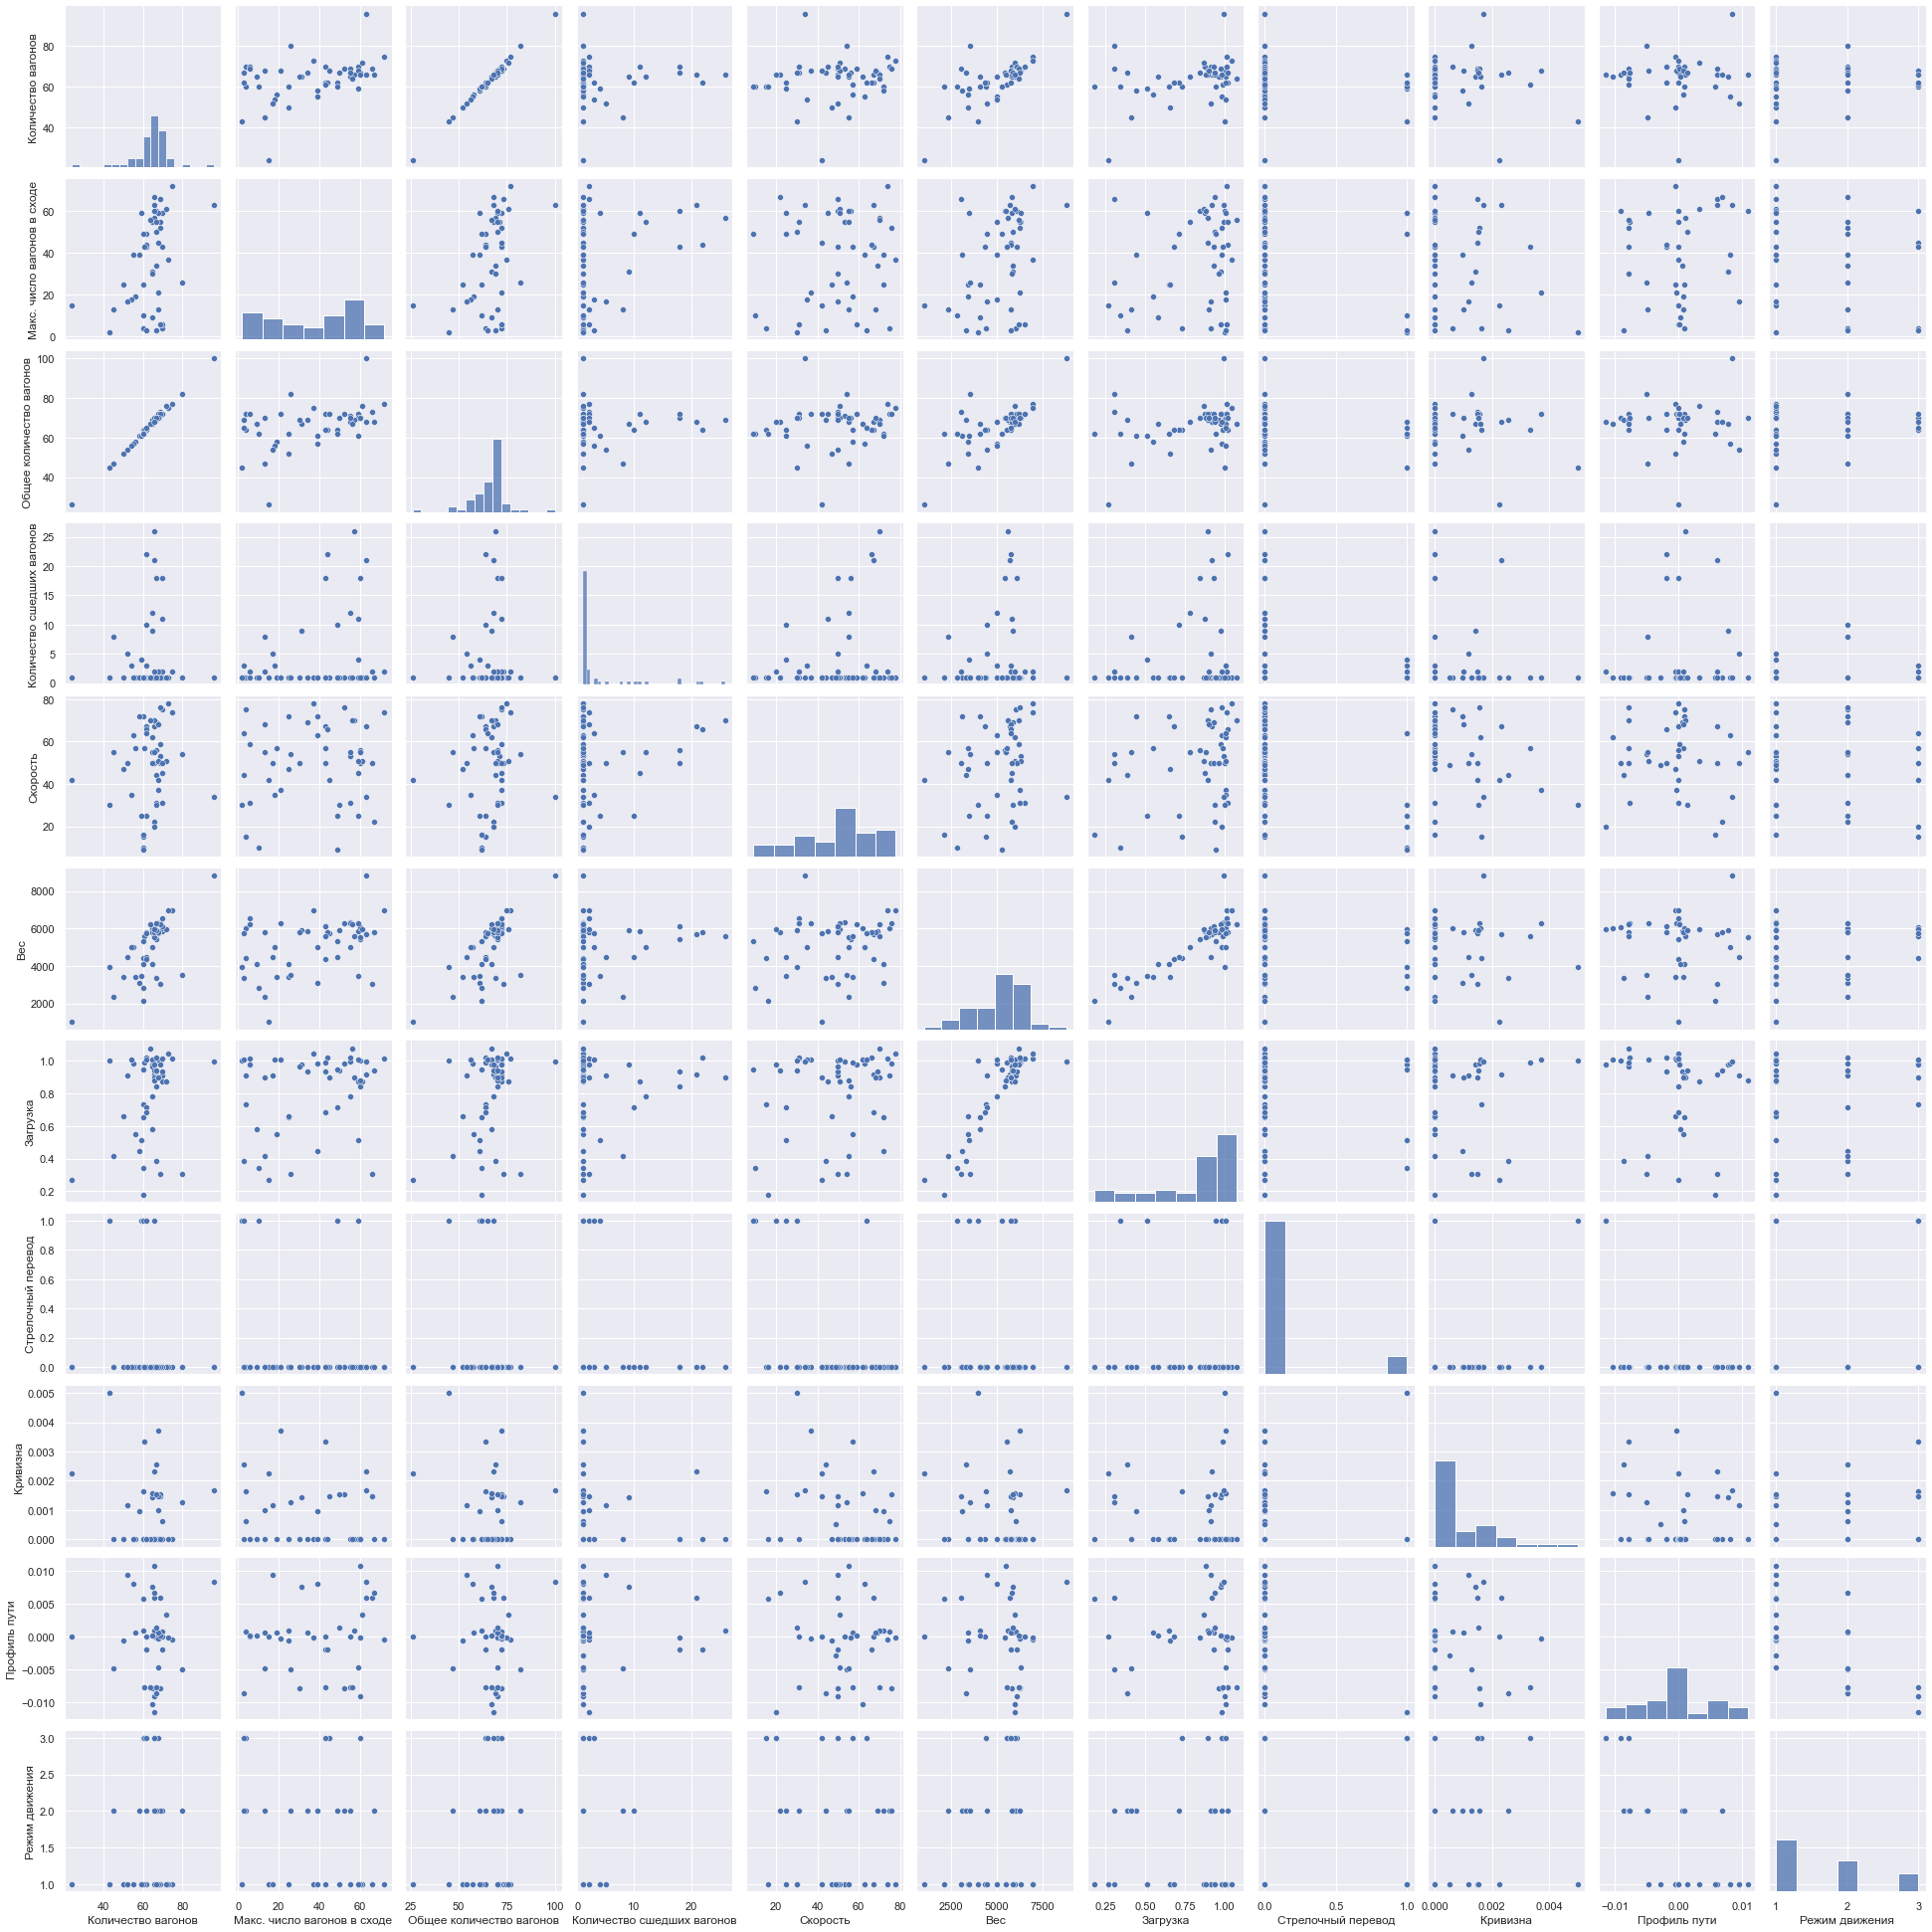
\includegraphics[width=1.0\linewidth]{src/img/pair_plot.png}
\caption{Пары признаков}
\label{fig:pair_plot}
\end{center}
\end{figure}

Изучив таблицу с описательными статистиками \ref{tab:basic_stats}, а также при детальном рассмотрении графиков пар признаков и распределений на рисунке \ref{fig:pair_plot} сильных выбросов в данных обнаружить не удалось.



\section{Оценка плотности распределения}

Построим ядерную оценку плотности распределения признака количества сошедших вагонов. В качестве ядра было взято стандартное гауссово ядро с шириной окна парзена $h = 0.5$.

\begin{figure}[H]
    \begin{center}
        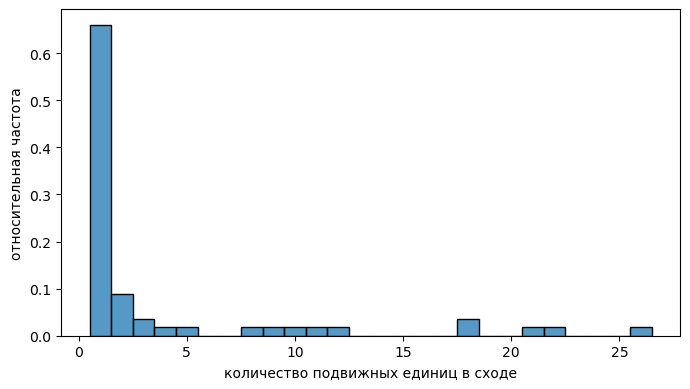
\includegraphics[width=1.0\linewidth]{src/img/KDE.png}
        \caption{Ядерная оценка плотности распределения}
        \label{fig:kde}
    \end{center}
\end{figure}

Из графика видно, что оценка плотности распределения признака количества сшедших поездов напоминает распределение Пуассона или геометрическое распределение.


